\documentclass[11pt]{article}
\usepackage{geometry}
\geometry{a4paper, left=25mm, right=25mm, top=25mm, bottom=30mm}

\usepackage{amsmath}
\usepackage{graphicx}
\usepackage{microtype}
\usepackage{parskip}
\usepackage{hyperref}

\title{Introduction to Neural Networks for Predicting Chaotic Systems}
\author{Sebastian M.D.}
\date{May 2024}

\begin{document}

\maketitle

\begin{figure}[h]
\centering
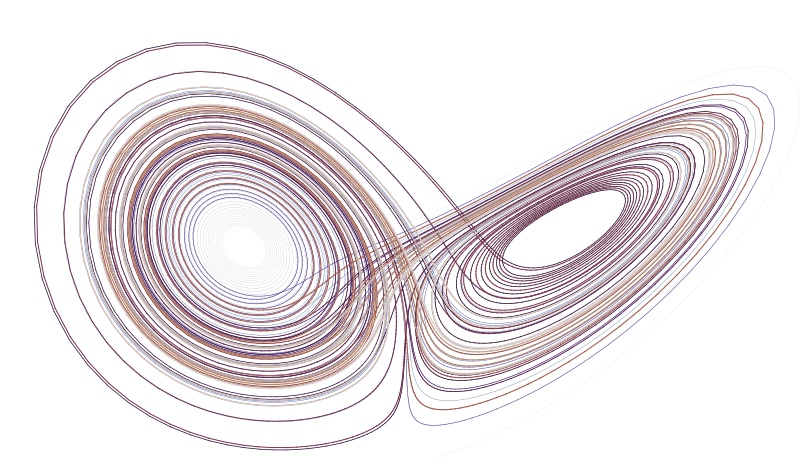
\includegraphics[width=0.4\textwidth]{title_page_image.jpeg}
\end{figure}

\section{Introduction}

Chaotic systems are deterministic systems which are highly sensitive to initial conditions, making long term predictions challenging. One such system aimed to model atmospheric convection is called the Lorenz 63 system, envisioned by Edward Lorenz in 1963. Traditionally, numerical methods have been used to predict these systems, but recent research has explored neural networks as an alternative solution. This is a summary of the paper: "Which Neural Network Architecture is Optimal for Predicting Chaotic Dynamics?" \cite{neural-network-comparison}. 

\section{Theory}

\subsection{The Lorenz System}
The Lorenz system is a set of three mathematical equations defined as follows:

\[
\frac{dx}{dt} = \sigma(y - x), \quad \frac{dy}{dt} = x(\rho - z) - y, \quad \frac{dz}{dt} = xy - \beta z
\]
In these equations, $x$, $y$, and $z$ are variables that change over time, and $\sigma$, $\rho$, and $\beta$ are constants. The equations create a pattern called the Lorenz attractor, see figure \ref{fig:lorenz_attractor}. This pattern looks like a butterfly's wings and shows how the system evolves over time. Even though the system is determinstic, its behavior is highly sensitive to initial conditions, meaning that a small change in initial starting values $x$, $y$, $z$, can lead to radically different $x$, $y$, $z$ values after a certain $t$ timesteps. 

\begin{figure}[h]

\centering
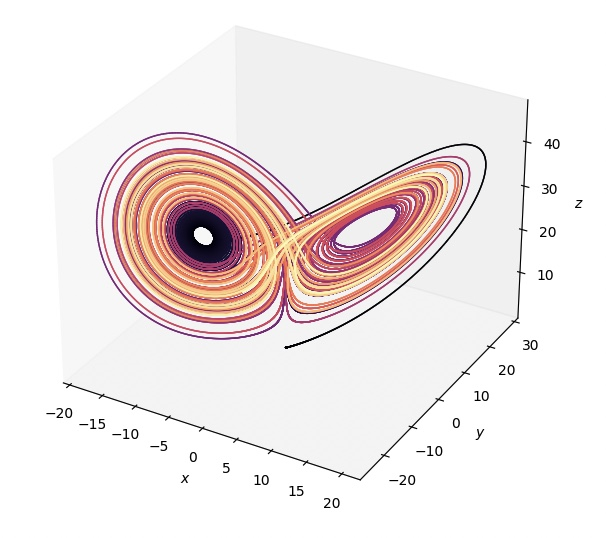
\includegraphics[width=0.3\textwidth]{lorenz_attractor.jpeg}
\caption{The Lorenz attractor visualized for 100 time units with $dt=0.04$}
\label{fig:lorenz_attractor}
\end{figure}

\subsection{Neural Networks}

Neural networks are a type of machine learning model inspired by how the human brain works. They consist of layers of interconnected nodes, which act like neurons, processing input data to produce an output. The connections between these nodes have weights and biases, which are parameters that decide what will get passed to the next node. The network starts with randomly set parameters, then by measuring the error in its predictions it will make small adjustments to these parameters that minimize the error. Mean Squared Error (MSE) is commonly used to detemine the degree of error in regression tasks. By adjusting the parameters in this way, the neural network learns to make accurate predictions on new, unseen data over time.


\subsection{RNNs}

A Recurrent Neural Network (RNN) is a type of neural network designed to recognize patterns in sequences of data. Unlike traditional neural networks, RNNs have connections that form loops. This allows them to maintain a 'memory' of previous inputs, which helps in processing sequential data like the Lorenz system. Long Short-Term Memory (LSTM) networks is variant of RNNs with improved capacity to 'remember' long-term dependencies and is used in this study.  

\subsection{Transformers}
Transformers are a type of neural network introduced in the paper "Attention is All You Need" \cite{DBLP:journals/corr/VaswaniSPUJGKP17}. Unlike previous models, they don't read data step-by-step but process the whole sequence at once. The key idea in Transformers is the self-attention mechanism. Each token in a sequence is turned into three vectors(three lists of numbers). The self-attention mechanism compares these vectors to find out how much each token should pay \emph{attention} to the others, thus finding the relationships between individual data points in a data sequence. The attention mechanism is usually applied in parallel blocks that form a layer. These layers are repeated a set number of times to form the full transformer network. 

\subsection{Reservoir Computing}
Reservoir Computing (RC) is a type of RNN. The main idea is that only part of the network is trained, making it faster and solving some problems found in traditional RNNs. Echo State Networks (ESNs) are a popular example of RC. In ESNs, the network has a random, sparsely connected part called the reservoir. The reservoirs output is dependent not only on the input but also on it's previous output, creating a form a 'memory'. Only the output layer is trained, typically using a method like ridge regression.


\section{Method}
This project involves creating, training, and evaulating machine learning models using Python, the PyTorch library and the ReservoirPy library. The project's code is available on GitHub at: \url{https://github.com/SebCodesTheWeb/lorents-net}.

\subsection{Generating Data}

Data was generated using a numerical method called the RK4 method. This method simulates the Lorenz system with random initial positions, and then records and saves the positions of the system as it moves through time in a CSV file. This data was then used to train the neural networks.

\subsection{Setting up the models}
The LSTM RNN model was set up using PyTorch's inbuilt nn.LSTM class and the Adam optimizer was used to train the parameters. The Transformers model was also built using PyTorch and trained similiary to the LSTM RNN model. The ESN model was implemented using the ReservoirPY library and was trained with the inbuilt ridge regression optimizer.

\subsection{Hyperparameter Optimization}
Hyperparameters are parameters that control the training process of a neural network. Hyperparameters could decide things like the number of layers, learning rate, training time, and network size of the model. A library called Optuna was used to find the best hyperparameters for the Transformers and LSTM RNN models. It was trained for 100 iterations per model on four RTX 4090 GPUs.

\subsection{Evaluation}
Once the models were trained they were then evaluated by predicting 500 time steps of the Lorenz system and comparing the predictions to the RK4 method. To evaluate the models, their Lorenz attractor shape, predicted trajectory and MSE
was taken into account.

\section{Results}
\subsection{Lorenz attractor shape}
\begin{figure}[ht]
    \centering
    \begin{minipage}{0.32\textwidth}
        \centering
        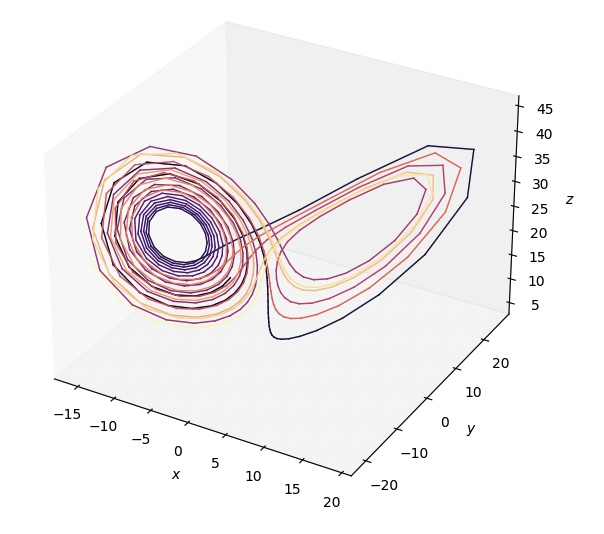
\includegraphics[width=\textwidth]{rnn_lorenz.jpeg}
        \caption{LSTM RNN}
        \label{fig:rnn_lorenz}
    \end{minipage}
    \hfill
    \begin{minipage}{0.32\textwidth}
        \centering
        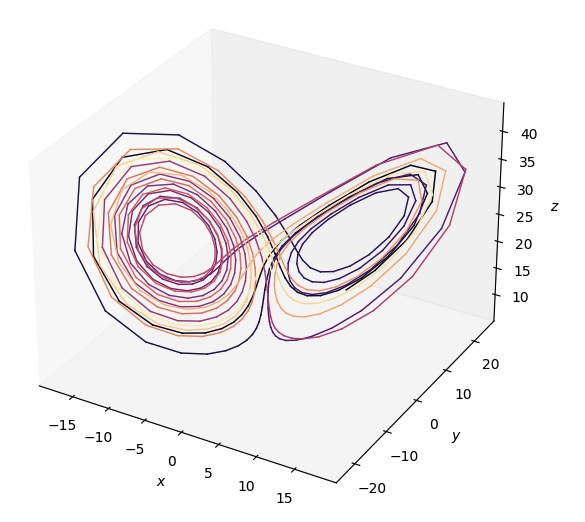
\includegraphics[width=\textwidth]{echo_lorenz.jpeg}
        \caption{ESN}
        \label{fig:echo_lorenz}
    \end{minipage}
    \hfill
    \begin{minipage}{0.32\textwidth}
        \centering
        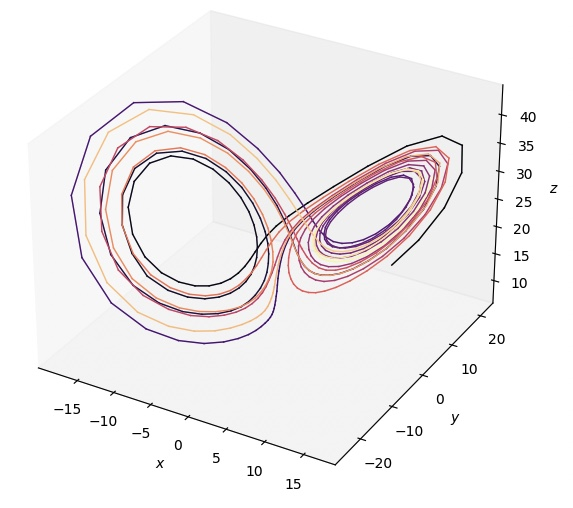
\includegraphics[width=\textwidth]{transformers_lorenz.jpeg}
        \caption{Transformers}
        \label{fig:transformers_lorenz}
    \end{minipage}
\end{figure}

\subsection{Predicted Trajectories}
View figures \ref{fig:rnn_path}, \ref{fig:echo_path} and \ref{fig:transformers_path} in Appendix A.
\subsection{MSE}
(Lower is better) \\
The average MSE for the LSTM RNN was 50.1579. \\
The average MSE for the ESN was 48.7797. \\
The average MSE for the Transformers network was 29.1590. 
\section{Discussion}
The figures show that all models have learned the Lorenz patterns, producing attractors with two wings around two focal points. However, there are differences in accuracy. The Transformers model and LSTM RNN models seem to have somewhat inaccurate proportions. The ESN model has better proportions between the two rings which are supposed to be of close to equal radius. Overall, the ESN model appears to have the most accurate Lorenz attractor shape.

The trajectory plots indicate different levels of accuracy. The LSTM RNN deviates from the true path around timestep 40-50. The ESN model diverges around timestep 60-100. The Transformers model divererges around timestep 100-120. Considering the input sequence lengths, the ESN can predict accurately for 70-80 timesteps, the LSTM RNN for 30-40 timesteps, and the Transformers model for about 60 timesteps.

\subsection{Conclusion}
The results suggest that the LSTM RNN was the worst performing model with the highest MSE and the shortest prediction accuracy. The ESN had the most accurate Lorenz attractor and the longest prediction accuracy, but the Transformers model had a lower average MSE. Although both the ESN and Transformers model show potential, further research is needed to optimize and compare these models conclusively. The study indicates however that the ESN is slightly better than the Transformers model, with the LSTM RNN being the least accurate.

Future research could explore the NVAR reservoir computing variant and further optimize ESN hyperparameters. For the Transformers model, experimenting with different positional embeddings and self-attention mechanisms could be beneficial. This could help determine the full potential of both the ESN and Transformers models in predicting chaotic systems.

\bibliographystyle{apalike}
\bibliography{references}

\appendix
\section*{Appendix}
\section{Predicted trajectories}
\begin{figure}
    \centering
    \begin{minipage}[b]{0.49\textwidth}
        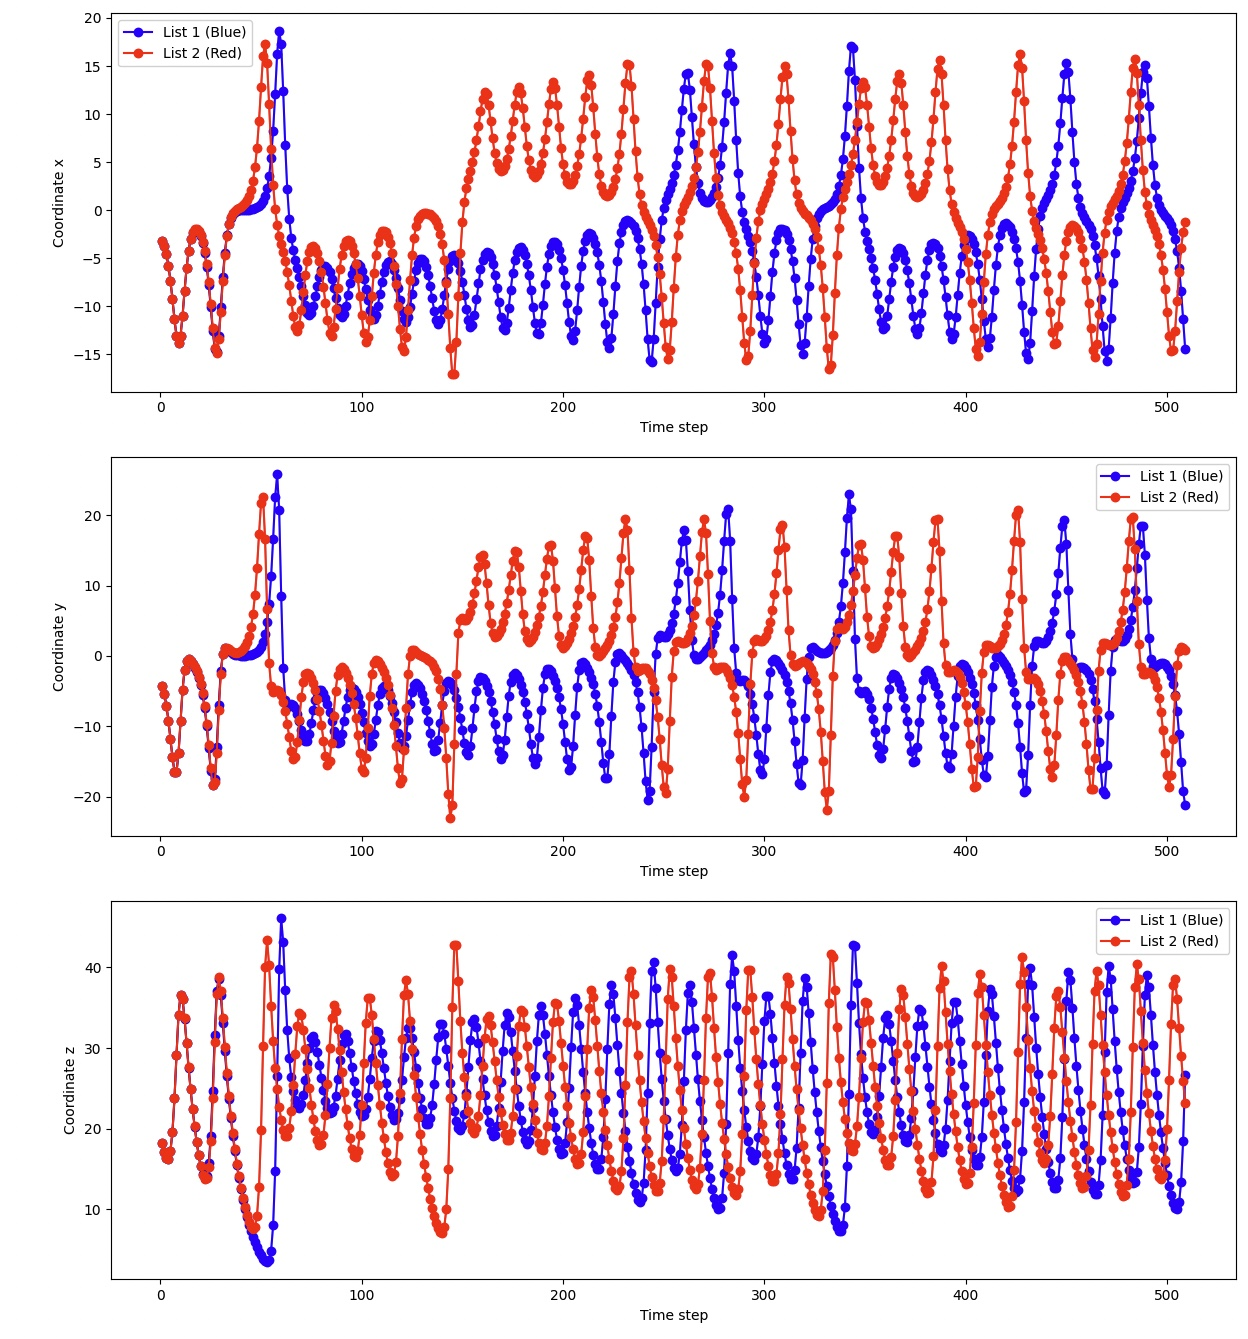
\includegraphics[width=\linewidth]{rnn_path.jpeg}
        \caption{LSTM RNN path (true path is red, model path is blue)}
        \label{fig:rnn_path}
    \end{minipage}
    \hfill
    \begin{minipage}[b]{0.49\textwidth}
        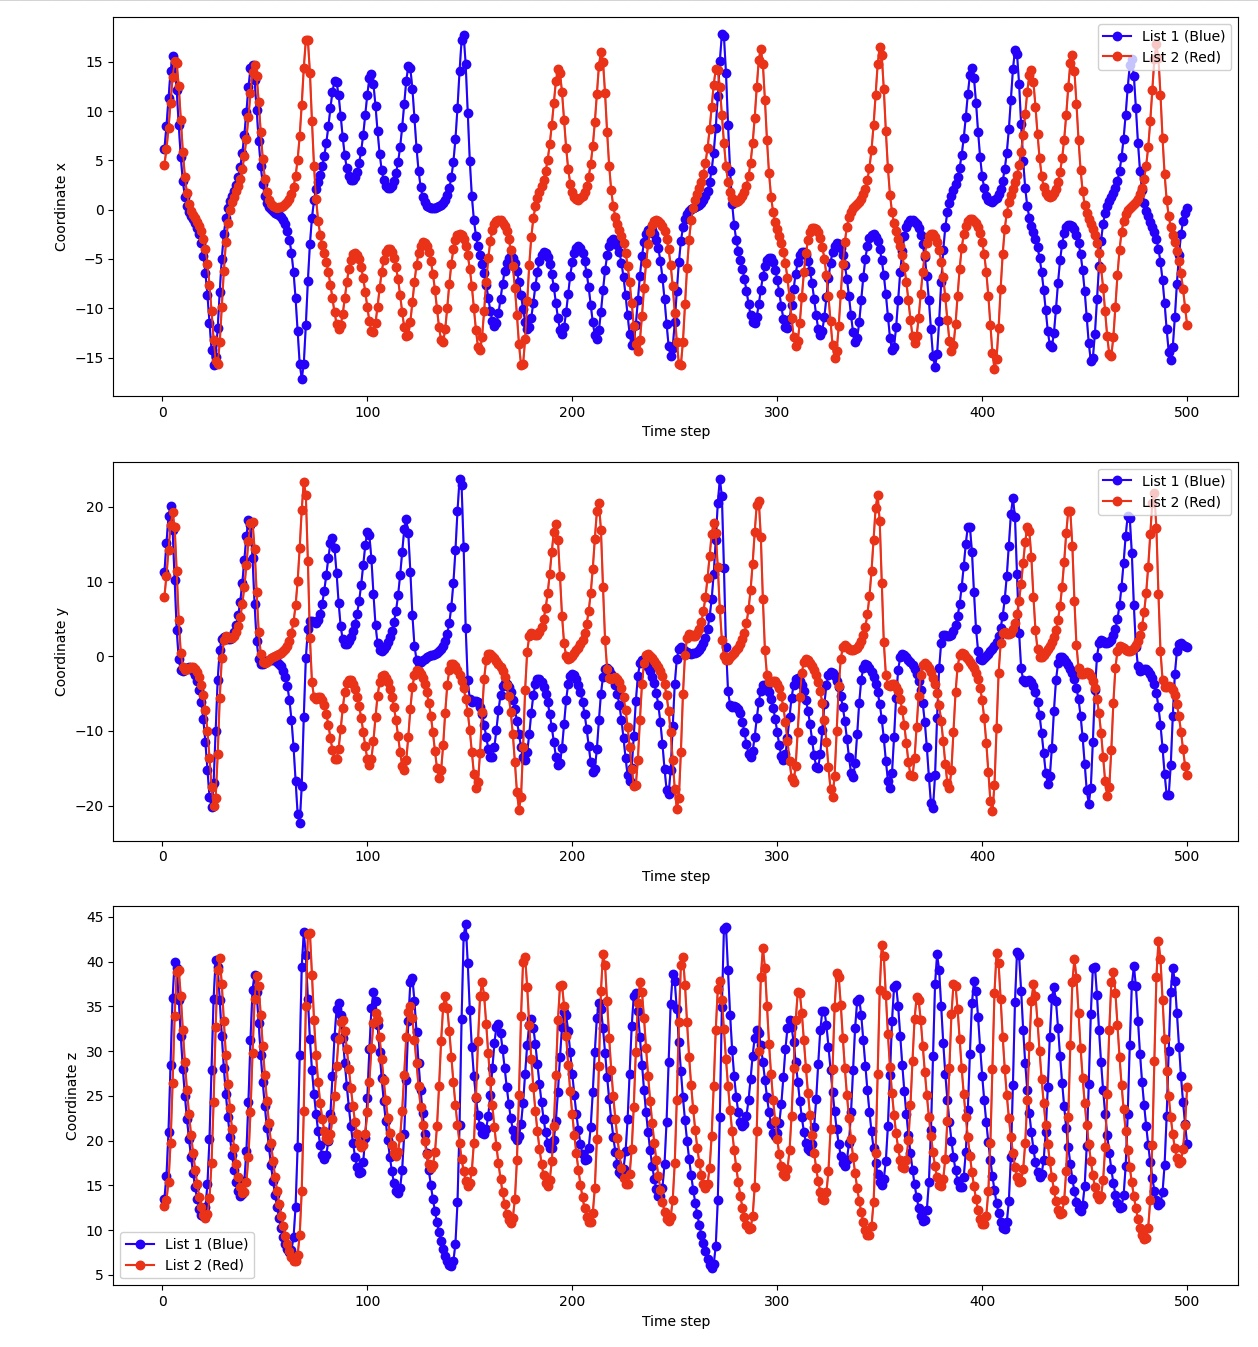
\includegraphics[width=\linewidth]{echo_path.jpeg}
        \caption{ESN path(true path is red, model path is blue)}
        \label{fig:echo_path}
    \end{minipage}
\end{figure}
\begin{figure}
    \centering
    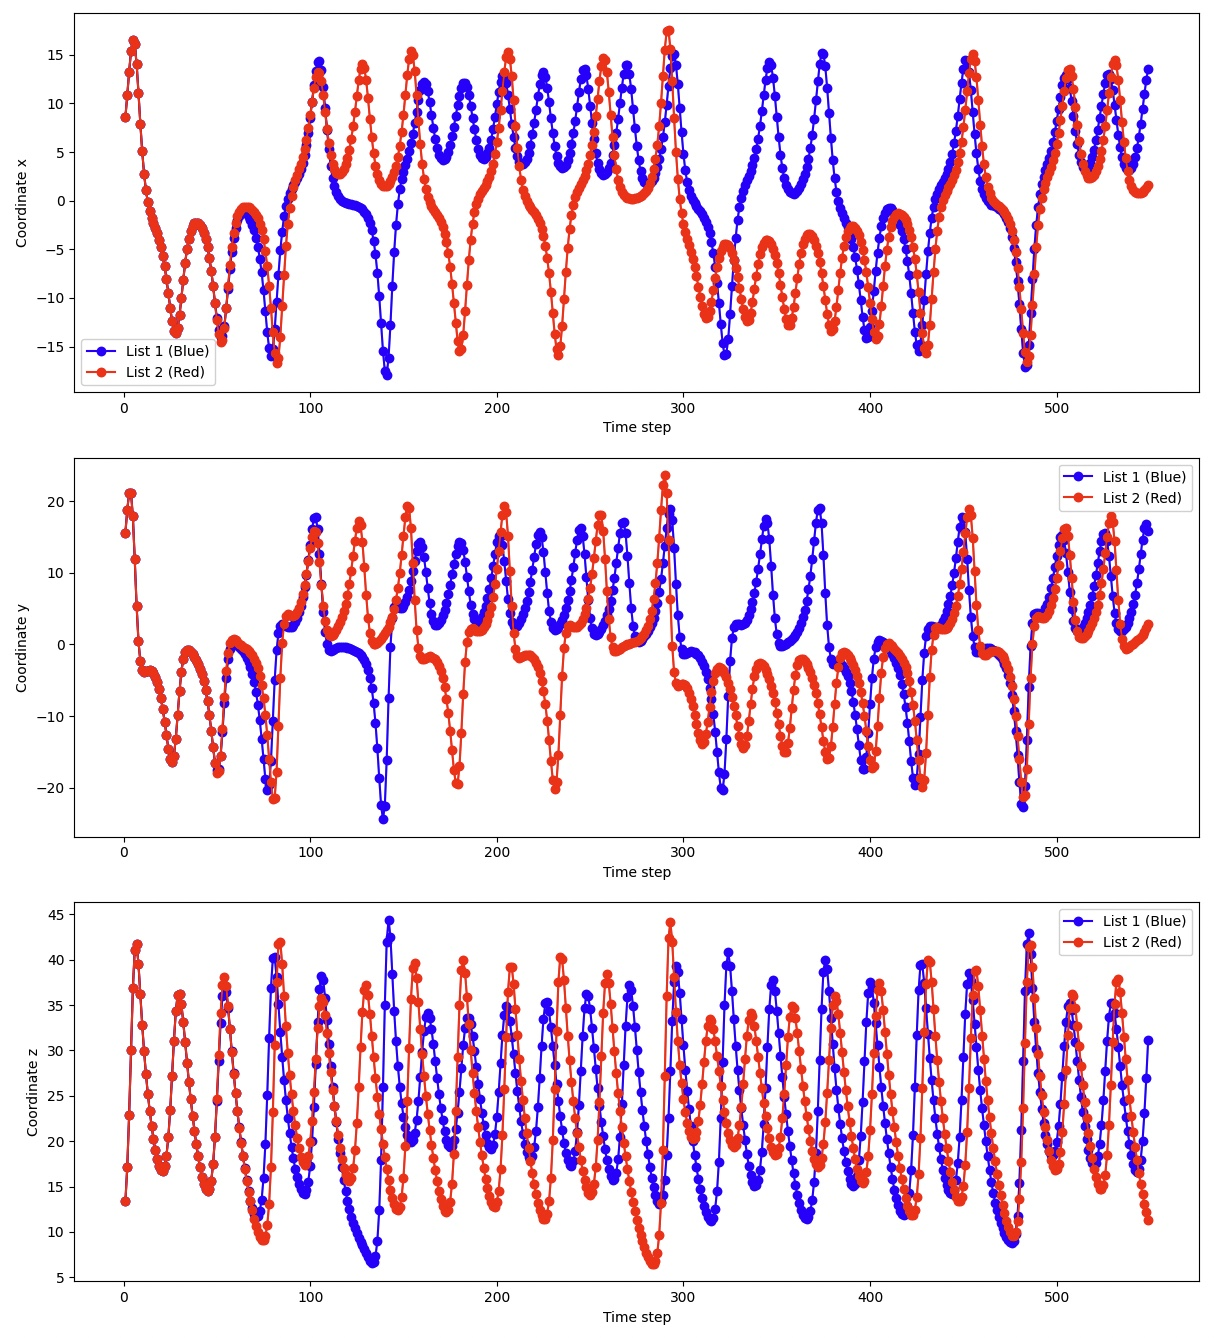
\includegraphics[width=0.6\textwidth]{transformers_path.jpeg}
    \caption{Transformers path(true path is red, model path is blue)}
    \label{fig:transformers_path}
\end{figure}


\end{document}
